\documentclass[a4paper]{article}
\usepackage{geometry, graphicx, url, float, rotating, algpseudocode, setspace}
\newgeometry{left=0.8in, right=0.8in, bottom=4cm, top=0.9in}
\onehalfspacing

%more interesting title?
\title{Using Twitter data to analyse people and their connections in a network - Progress Report}
\author{Caroline Player 1112108}
\date{}

\begin{document}

\maketitle
\pagestyle{plain}

\section{Introduction}
This report documents the progress of a 30 week project which aims to take a sample of Twitter and represent the users in a unique way. Currently, this project is nine weeks into the schedule and a refactored Gantt chart for the project is discussed below. This document discusses implementation from the past nine weeks, as well as looking at the design of systems yet to be developed. 

\section{Project Aims}
This project aims to represent unique analysis of Twitter users. The project can be broken down into three main sections: data collection, analysis and visualisation. The data collection is subject to the constraints of how much data can be extracted from Twitter, this is known as the rate limit. This in turn, imposes a time constraint, as the application must wait a certain amount of time for the resources to be replenished. The analysis aims to consider users, categorise their interests, and compare the results to other Twitter users. The motivation behind this is we can then see why certain connections might exist in a network, and whether perhaps there are more relevant communities on Twitter that a user might benefit from being connected to. Finally, this analysis needs to be visualised to those who wish to explore the results. 

\section{Design}
\begin{figure}
	\centering
	     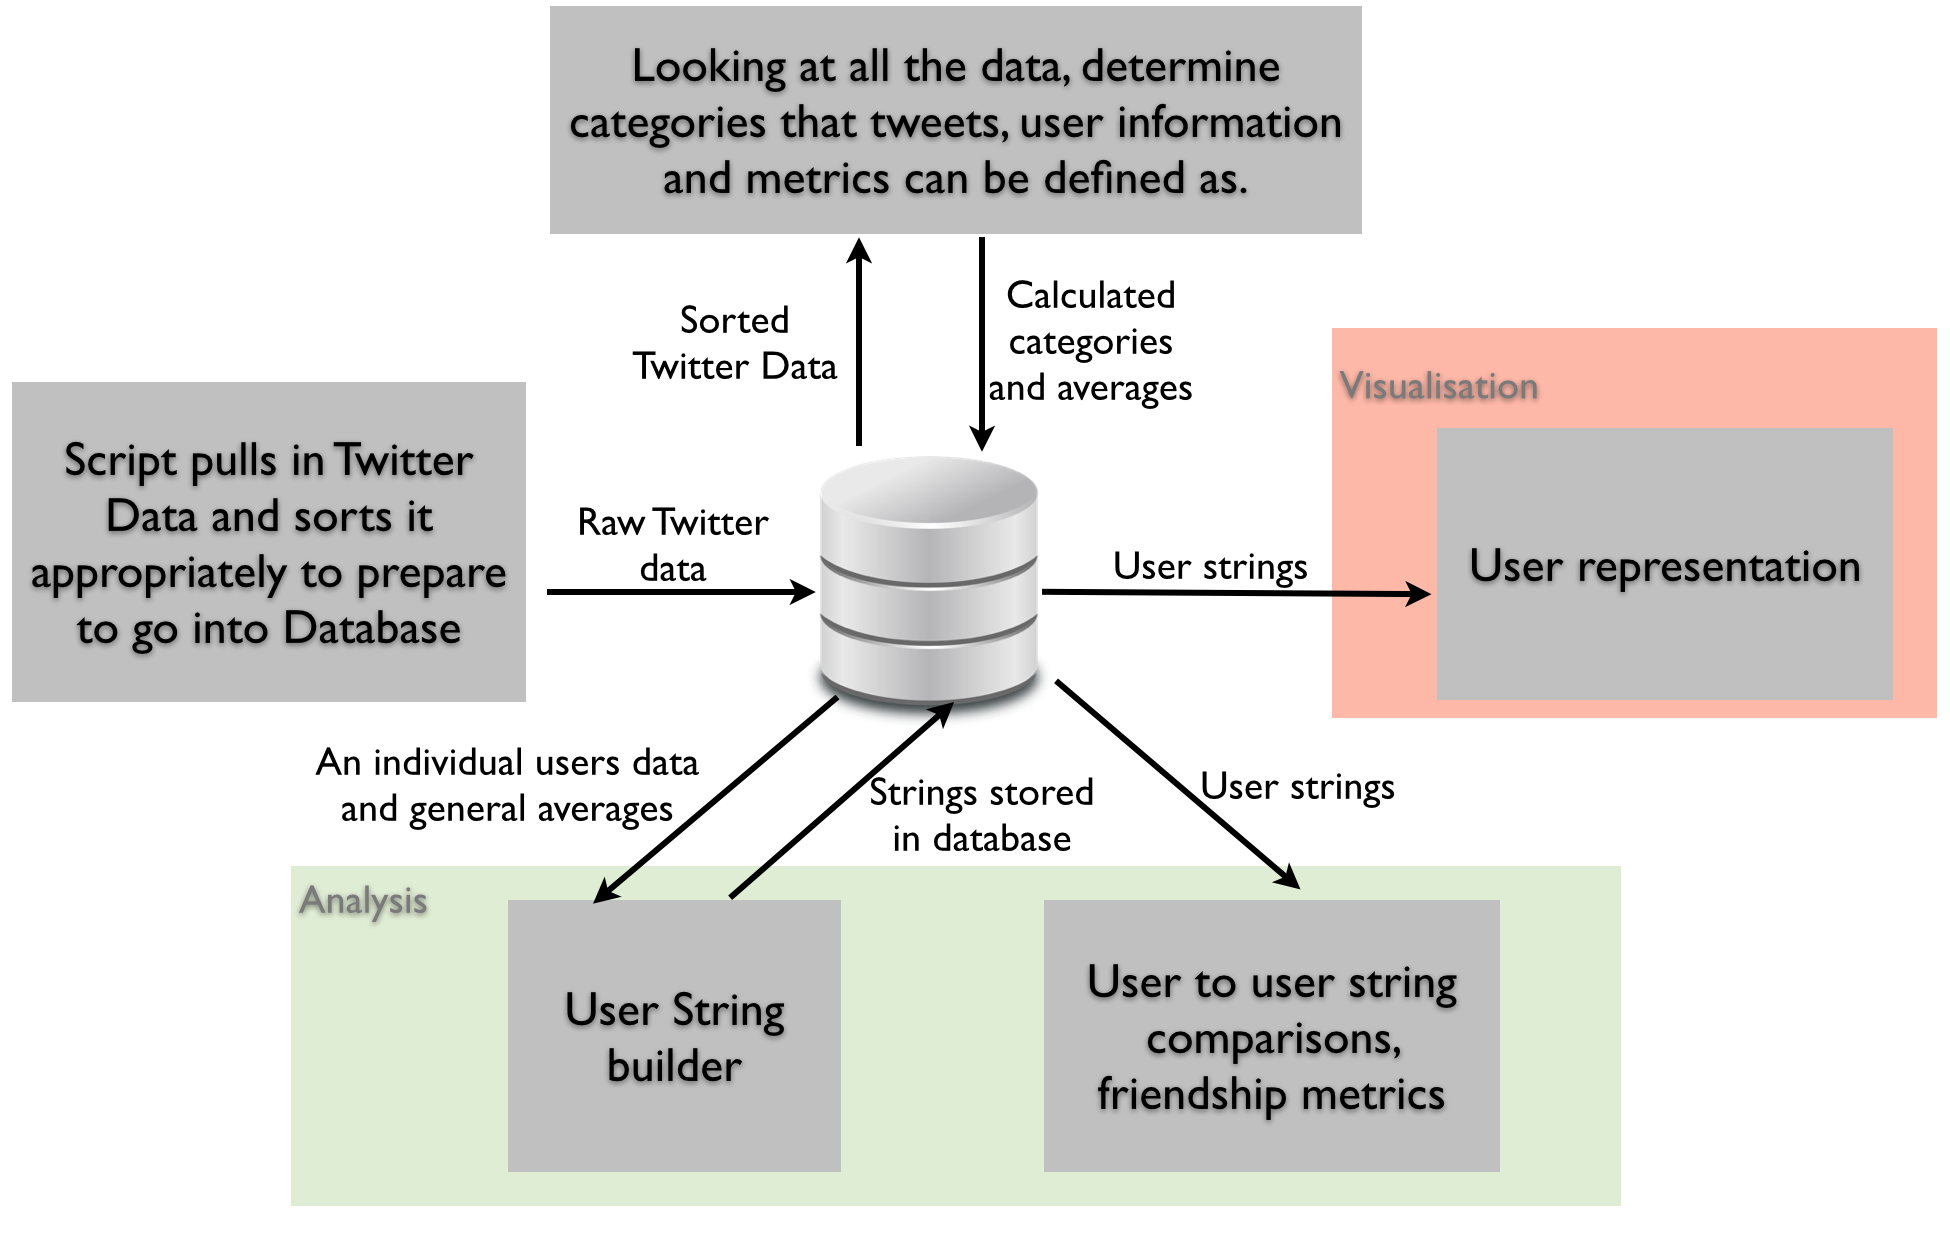
\includegraphics[scale=0.45]{architecture.png}
	  \caption{System architecture.}
	  \label{fig:arch}
\end{figure}
Since the initial specification of nine week ago, there has been implementation of data collection and certain amounts of refactoring to the system design. An updated image of the system architecture can be seen in Figure~\ref{fig:arch}, from the original design in the specification document. This is due to the availability of data, limitations of APIs and time constraints. Design decisions for the various sections of the system are discussed below. Section~\ref{subsec:designcrawlingtwitter} discusses design of systems already implemented, however section~\ref{subsec:designanalysis} is yet to be implemented and so the design is the current plan discussed in Section~\ref{sec:futurework}, and the time schedule for this development will follow the Gantt chart in Figure~\ref{fig:gantt}.
\subsection{System Design}
Figure~\ref{fig:arch} displays the design for the system architecture. It is slightly different from the design of the specification document as nine weeks in the project scope is slightly more defined and time constraints have shown what is feasible for completion during the rest of the project. The data collection is stored in the database, which is then pulled out by the analysis engine for building a representation of the user we call user strings. The strings are then used for more analysis on Twitter users and their connections. Finally, this all needs to be visualised and so the analysis is stored back into the database and pulled out be the software which aims to visualise all this data and analysis.
\subsection{Crawling Twitter}
\label{subsec:designcrawlingtwitter}
To allow for a fair representation of users and the network, the data the analysis is being based on needs to be as representative of the Twitter network as possible. At the same time we cannot gather too much information on one user because the application is subject other resource limitations of the API, and to compromise we get what is minimally required for the analysis we hope to undertake in order to get information on more users.\\
The code is currently designed to start at a random Twitter user. The details of this user are requested from Twitter, and appropriate attributes of the user are stored to the database. If the user has not been seen before then a large amount of tweets are grabbed. This is because given the 555 million Twitter users~\cite{twitterstat}, that one user is unlikely to be visited again and we need a high threshold of tweets to base analysis on. The user may have been visited before though, in which case we grab less tweets so as to not use up too much of the resources allocated to the application in the current fifteen minute window, but we know that we previously grabbed a larger amount of tweets, and are now just increasing the quantity of data to analyse them, which should make the analysis more reliable is it gives a wider overview of the user.\\
When a user is being added to the database, we want to collect many of their friends and followers on Twitter without using too many of the resources. Once friends, followers, tweets and user information have been saved, we can move on to find the next user. It is important that the next user be chosen not entirely at random because otherwise we would find ourselves requesting data on a very popular Twitter user much more often than we need to. For example, Stephen Fry has six million followers, where as a quiet imaginary user has just one follower. When we crawl Twitter and need to move onto a user, there are six million possible users that could lead us to Stephen Fry, while there is just one that can lead us to our hypothetical user. But we know from just one visit to Stephen Fry that he is a popular Twitter user because we grabbed certain information on him that told us that, such as how many followers he has and how many tweets he has made. So visiting him a few more times to get more tweets from him will be useful, but we do not want to visit him six million times more than our hypothetical user. So we cannot select random neighbours of our current user and move on. The next user is selecting following the Metropolis-Hastings Random Walk algorithm discussed in section~\ref{sec:implementation}.
\subsection{Analysis}
\label{subsec:designanalysis}
Now that the relevant raw data is stored in the database we can start to associate meaning to a users information. We have the hashtags from users, and their metadata, but unless we do sentiment analysis on the text, and quantitative analysis on the whole graph we will not be able to judge what makes a user influential in the network, or a sporty or academic person. By running the tweets of a user through sentiment analysis we aim to understand their interests and feelings. Each user will be assigned a string which consists of a series of binary bits, where a one represents an indication the user is interested in or has a certain characteristics of the category that index in the string represents. We know that just sentiment analysis cannot be considered, which is why during data collection we are interested in more than just the content of a tweet~\cite{BravoMarquezF2013Combining}. Categories for example may consist of Sports, Academic, Music, TV, Unusual Hobbies, Vocal, Celebrity. So a user who is sporty will get a one as the first bit, but who does not have intellectually stimulating hobbies might get a 0 in the academic category, as an example a string might look as follows: 1001011, where this user could be a famous footballer who also likes to talk about what they are currently listening to. From this we can see that we need sentiment analysis on the users tweets to determine their interests, but this is not enough. Several categories can be considered when analysing a user on Twitter. From a particular paper designed at categorising users into their sector such as company, government, celebrity~\cite{hashtagwearefollowers}, we learn we need to consider how many times tweets are retweeted, favourited, what types of users retweeted them, additional content within the tweet, hashtags, statement types (these can include announcement, declarative, draw-the eye, idle chatter and many more) and finally if the tweet is a question. We can apply this research by using these indicators to decide whether bit is our user strings are given a one or a zero.

\section{Implementation}
\label{sec:implementation}
Thus far in the project, the Ruby script which uses the Twitter API to gather Twitter data in an unbiased manner has been implemented, and the analysis is yet to be applied. The following subsections describe the implementation details of crawling Twitter. 
\subsection{Metropolis Hastings Random Walk algorithm}
For this project, using the Twitter sample stream is unacceptable as we need to control which users we grab information on, for reasons described in section~\ref{subsec:designcrawlingtwitter}. Therefore the Ruby script which has been implemented for this project needs to consider the following things:
\begin{itemize}
\item Firstly, we want more than just tweets, we would like information on the user that tweeted it, whether it was a retweet and who was the original author of that retweet.
\item Secondly, we cannot guarantee that the stream twitter provide is a fair representation of the Twitter network. Understanding that the Twitter network is far too large to download~\cite{twitterservers}, we need to take a representative sample. 
\item Finally, the difference between uni-directional and bi-directional social network graphs where nodes are users and edges represent relationships needed to considered. The difference can be seen in a Facebook friend which is a mutual friendship compared with a Twitter follower where the person being followed is not required to reciprocate the relationship. These are called unidirectional and bi-directional graphs respectively, and we need to unbiasedly sample a bi-directional graph as well as possible. 
\end{itemize}
The Metropolis Hastings Random Walk (MHRW) algorithm treats uni-directional graphs as bi-directional graphs~\cite{MHRWunidirectional}~\cite{bidirectionaltrawling}.So we discount the fact that some edges come into a node and that some come out, and consider them all as bi-directional. We then choose one of the neighbours that these edges go to at random, and consider it's degree (how many edges it is connected to). We can calculate a ratio which is the degree of the current node over the degree of the neighbour node and compare it to a random decimal number between zero and one. If the random number is less than or equal the ratio we update the current node to be the neighbour, and so we have moved round the graph. This means that if the current node has a higher degree than the neighbour node, that neighbour node will always be chosen, because the ratio will be higher than one and p cannot exceed one. If the neighbour node has a higher degree then we need to be more careful about whether we go there, because the reason for using this algorithm is to avoid overly popular nodes and give other users a chance to be visited even just once, but we do still occasionally want to visit those popular nodes. So the ratio will depend on just how popular the other neighbour is, and the random number means that sometimes the ratio allows us to visit that popular user, but not always. We then repeat the algorithm with our update current node. This can be seen as pseudocode below in section~\ref{subsec:pseudo}.
\subsection{Twitter API}
The Twitter API allows access to all the public data on Twitter, albeit with resource limitations. The script which runs the data collection uses a wrapper around this API to provide simplicity in the code. The wrapper is a Ruby library for the Twitter search and REST API found on GitHub~\cite{sferik}. 
\subsection{Data Collection}
Gathering Twitter data is subject to rate limits and permissions of the user trying to collect the data. As a stand-alone application, which my project is considered to be, I am entitled to the minimum amount of data the Twitter API will provide, the most limiting factor of which is 180 user requests every fifteen minutes. Therefore the process of collecting a substantial amount of data is subject to a time constraint where I must gather what data I can within the resources available to me, then wait for fifteen minutes until the resources are replenished.
Gathering more than just tweets is important because in the analysis section, we want to evaluate characteristics of the user as discussed in section~\ref{subsec:designanalysis}. This data is gathered by selecting the following information to store in the database: user's id, screen name, how many people they follow, how many people follow them, how many tweets they have made, the tweets, the hashtags they have used and the ids of the people who follow them and who they follow. The data is stored in a MySQL database because the Ruby language which is being used to gather Twitter data also has an extensive MySQL library, making it easy to interface with the database.\\ 
Other information stored in the database are cursors. Cursors were implemented in version 1.1 of Twitter as a way of paging through long lists that could potentially be returned by a request, for example asking for all of Stephen Fry's six million followers. Should you have unlimited access to data and not be rate limited, then this would be returned in several pages of ids, where at the end of the page is the cursor that points to the next page of data. To use this to our advantage in rate limiting we can store the next cursor with the users information. So if we revisit that user, instead of grabbing all the same followers, we request the value for the cursor that points to the next page of followers, and request that. 
Similarly with tweets, to avoid grabbing all the same tweets, Twitter allows you to input arguments when requesting the stream of a particular users tweets which are called since\_id and max\_id. These specify the most recent tweet we requested, and the oldest respectively. Then Twitter will only return tweets newer than the id of since\_id, should there be any new tweets, and from there historical data passed the tweet whose id is the same as max\_id. 
\subsection{Data collection algorithm} 
\label{subsec:pseudo}
The following pseudo code explains how data is collected and stored to the database. The justification for values and the user of the MHRW algorithm is explained above.\\
\begin{algorithmic}
\Function{main}{}
	\State $current\_id \gets random\_id$
	\While{current\_id not null}
		\State getData(current\_id)
		\State $neighbour\_id \gets randomNeighbourNode$
		\State $current\_id \gets MHRW(current\_id, neighbour\_id)$
	\EndWhile
\EndFunction\\

\Function{MHRW}{current\_id, neighbour\_id}
	\State $p\gets ~random(0..1)$
	\State $ratio\gets $ $\frac{current\ neighbour\ count}{neighbour\ neighbour\ count}$\\

	\If {$p\leq ratio $}
		\State $current\_id \gets neighbour\_id$
	\Else{}
		\State current\_id remains the same
	\EndIf
\EndFunction\\

\Function{getData}{current\_id}
	\State add or update user metadata
	\If {$new\ user$}
		\State grab 100 tweets
		\State store cursor values
		\State grab up to 5000 followers and 5000 friends
		\State store cursor values
	\ElsIf {$revisiting\ user$}
		\State grab 50 tweets using cursor values
		\State grab up to 5000 followers and 5000 friends using cursor values
		\State update cursor values
		\State update data on perviously stored tweets
	\EndIf
\EndFunction
\end{algorithmic}

\section{Future work}
\label{sec:futurework}
Nine out of thirty weeks of the project have now elapsed, and the first element is completed, as discussed above. The remaining time is to be spent on the analysis and visualisation of the data. The time plan visualised as a Gantt chart for the upcoming 21 weeks can be seen in Figure ~\ref{fig:gantt}. The deadline for the report is week 30, but it should be noted the project should be at completion by week 25 for a presentation.
\begin{sidewaysfigure}
	\centering
	     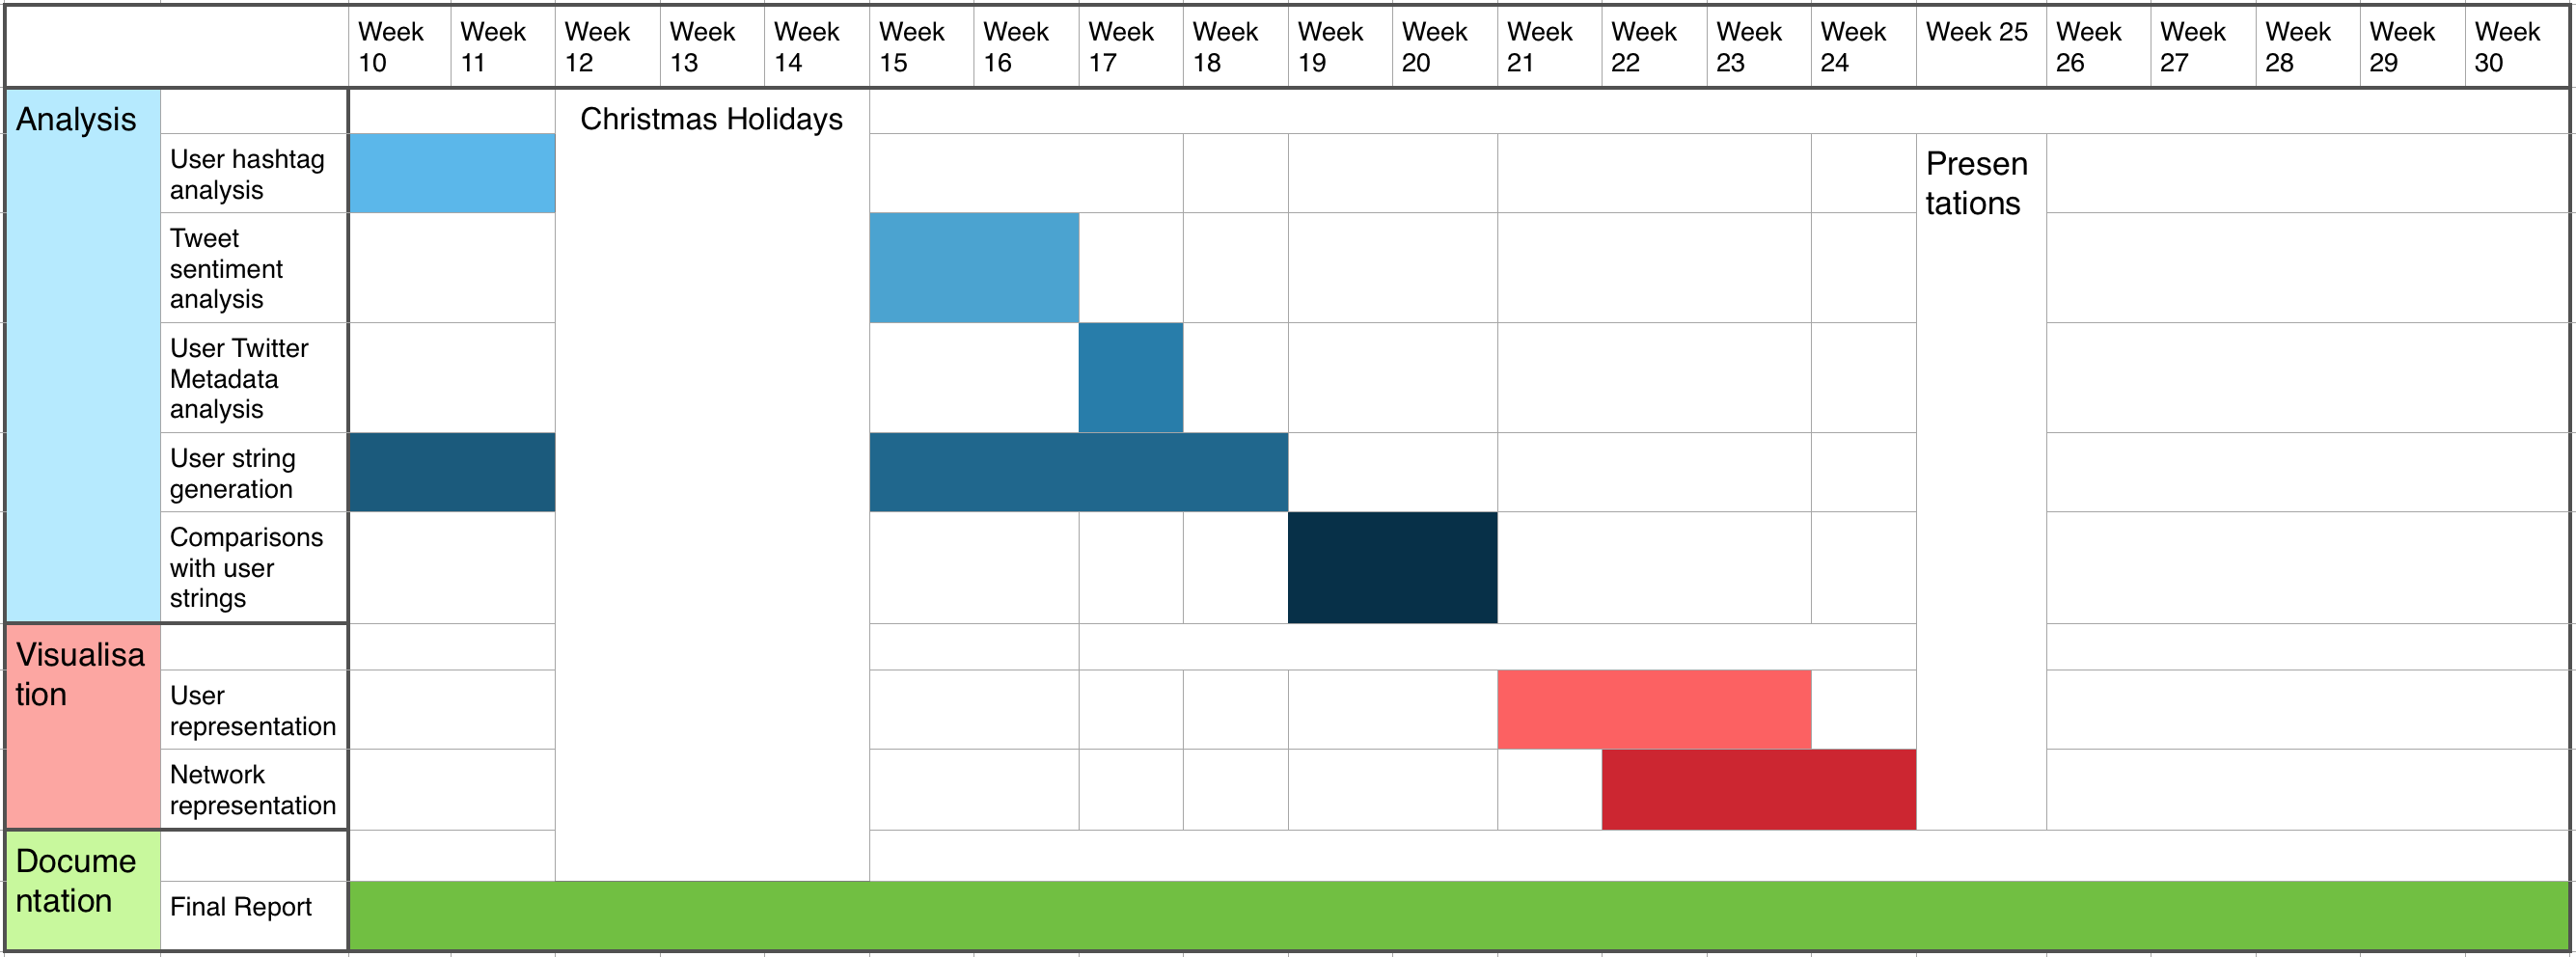
\includegraphics[scale=0.5]{ganttchart.png}
	  \caption{Gantt Chart.}
	  \label{fig:gantt}
\end{sidewaysfigure}
The justification of this Gantt chart can be seen in the following subsections for each of the three remaining categories to be implemented over the next twenty weeks.
\subsection{Data collection}
While the script to collect data has been written, due to the rate limit of Twitter this needs to be left running for a significant amount of time. This will be done by running the script on Joshua, which will allow for it to be collected 24 hours a day, and also means I can ssh in to the network to check that it is still running properly. This can be left running while I develop analysis because as development goes on I can apply the analysis to a bigger and bigger dataset. The script will be moved onto Joshua within a week, because a few days still needs to be taken to test the script.
\subsection{Analysis}
The analysis of the project can be broken down into the five stages seen in Figure~\ref{fig:gantt}. These tasks have been discussed along with their design in section~\ref{subsec:designanalysis}. A refactoring of time management has suggested there will not be time in the project for network analysis. Generating user strings and doing user comparisons will fill the rest of the twenty weeks. This project has scope for much analysis, not all of which is feasible to accomplish in the time frame. 
\subsection{Visual representation}
While user strings can be seen if queried from the database, this is not a good visualisation of the analysis. We would like to implement a system which shows the user string, the similarities in strings between their friends and followers and perhaps people in the network who are very similar that they might benefit from being connected to.
\subsection{Documentation}
The final report associated with this project is due in the last week. As work is being done over such a long period of time, the most accurate documentation of the project will come from it being written throughout the development. Therefore the appropriate sections will be written just after a task is completed and why the final report in the Gantt chart in Figure~\ref{fig:gantt} spreads across the entire timeline.

\section{Testing}
Testing needs to be carried out throughout the development. As the project is being developed in the Integrated Development Environment (IDE) Eclipse, with the appropriate development tools plugged in, there are unit tests provided. Because of the iterative development, building the script to grab data was built up in such a way that the additions to the code were tested alone and once working, tested with the whole system. As the system built up, black box testing was undertaken, which ensure the desired results were being stored in the database. Regression testing was also taken into account. Sometimes the Twitter API or the Ruby wrapper to the Twitter library I was using did not work seamlessly, and so backtracking and work arounds had to be implemented. However as mentioned before, the next important step was not built until the current one was working properly. This type of testing will continue throughout the remainder of the project.

\section{Evaluation}
At the end of the project, users should all be associated with strings that represent them. We can compare a user to another by comparing the strings and finding the similarities. We understand that Twitter sentiment analysis is a developing research area and that there are many more factors to be considered in a person than what they make public on Twitter, therefore we cannot take the analysis as it is planned too seriously because as these technologies develop, so will the quality of the results produced by this project. We can take from this project though that users will have this unique representation which can have more analysis applied to it as well built up in a more detailed manner than what this project aims to complete. 

\section{Conclusion}
A lot of progress has been made now that it is a third of the way into the project. The data collection has been implemented successfully, though the scope of the project has been narrowed down to fit the time scale more appropriately. As a result of the implementation already completed and the design of the rest of the system as discussed in this document, the project aims to continue to be as successful and finish on time.

\bibliography{bibliography}
\bibliographystyle{plain}

\end{document}